\begin{frame}[fragile,label=ss-approach] 
\secframetitle{\ssApproach}
\framesubtitle{\enzo's limitations}
%\framesubtitle{Scaling issues}
\begin{minipage}{3.0in}
%  AMR data structure scalability
%  Code development and maintenance
%  Ghost zone memory requirement
%  Patch size variation
%  Time stepping
%  Dynamic load balancing
%  Particle positions
%  Mesh quality
% So, how does Cello's AMR try to address the know issues of Enzo's current
% AMR?
%
% The main issues with Enzo's AMR design and implementation involve
% memory usage, the quality of the mesh, parallel task definition
% and scheduling, and data locality.

% [MEMORY] Memory usage is perhaps the most common limitation that
% people run into when running big Enzo simulations.  Enzo's mesh
% hierarchy structure is represented in each MPI process using a
% grid object for each AMR patch.  Although patches assigned to
% remote processors carry no field or particle data, the grid
% objects themselves still take up on the order of a few KB of memory.
% For small hierarchies that's not a problem, but when you have a million
% grid patches that means several GB of memory are required on each
% MPI process.  While supercomputers have gotten larger over the years, the
% amount of memory per node has not---it's still frequently just a few
% GB.  :  Memory fragmentation has also been identified as a problem,
% due to the high volume of heap memory new and delete operations on
% widely varying array sizes.  Ghost zone data can also consume a lot
% of memory, especially for smaller grids.

% [ MESH QUALITY ] Enzo also has known mesh quality issues.  Sometimes
% patches are adjacent to patches in refinement levels that are further than 
% a factor of two different. This can lead to inaccurate interpolation
% compromizing the numerical accuracy of solutions on such patches.

% [ PARALLEL TASKS ] Parallel tasks in Enzo are defined as a grid
% object and its associated field and particle data.  Patch sizes in
% Enzo can vary widly, from large $64^3$ root grid tiles to small
% $8^3$ patches on the finest levels.  Varying task sizes can
% adversely affect performance and load balancing.

\begin{itemize}
\item \bfat{2}{\textcolor{red!50!black}{Memory usage}}
\begin{itemize}
  \item<2-> \textcolor{red}{AMR structure is non-scalable}
  \item<2-> \textcolor{red}{memory fragmentation}
  \item<2-> \textcolor{red}{ghost zones}
\end{itemize}
\item \bfat{3}{\textcolor{green!50!black}{Mesh quality}}
\begin{itemize}
   \item<3-> \textcolor{green!80!black}{2-to-1 refinement constraint violated}
\end{itemize}
\item \bfat{4}{\textcolor{blue!50!black}{Parallel task definition}}
\begin{itemize}
   \item<4-> \textcolor{blue}{widely varying patch sizes}
   \item<4-> \textcolor{blue}{sizes determined by AMR}
\end{itemize}
\item \bfat{5}{\textcolor{cyan!50!black}{Parallel task scheduling}}
\begin{itemize}
   \item<5-> \textcolor{cyan!80!black}{parallel within a level}
   \item<5-> \textcolor{cyan!80!black}{synchronization between level time steps}
\end{itemize}
\item \bfat{6}{\textcolor{orange!50!black}{Data locality}}
\begin{itemize}
   \item<6-> \textcolor{orange!80!black}{disrupted by load balancing}
\end{itemize}
\end{itemize}
\end{minipage} \
\begin{minipage}{1.0in}
\centerline{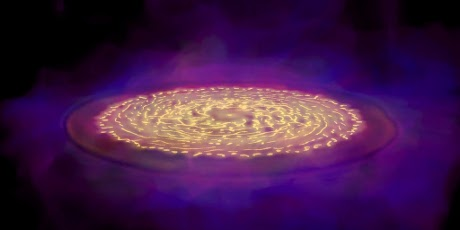
\includegraphics[width=2.0in,angle=90]{iso_and_volume_02_sm.jpg}}
\centerline{\tiny{[ Elizabeth Tasker ]}}
\end{minipage}
\end{frame}
